\section{Discussion}

\begin{figure}
  \centering{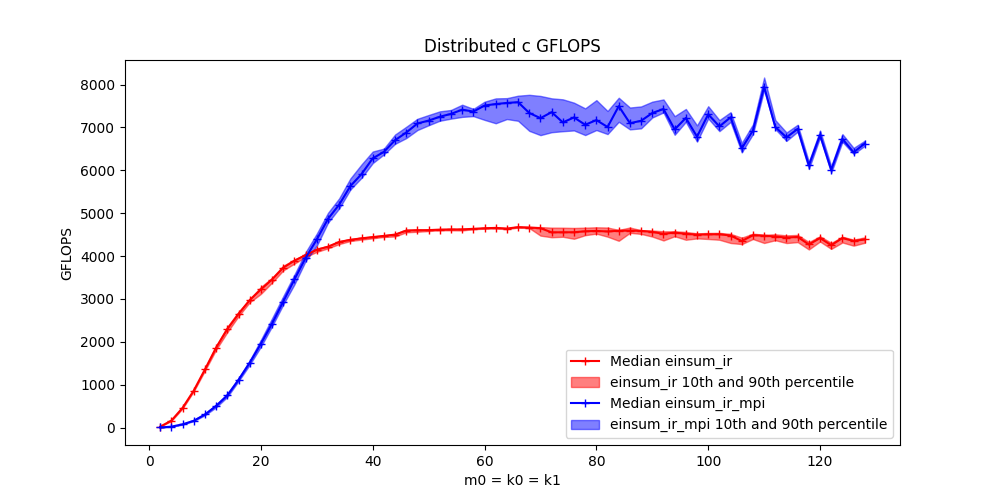
\includegraphics[width=0.95\textwidth]{gflops_c.png}
  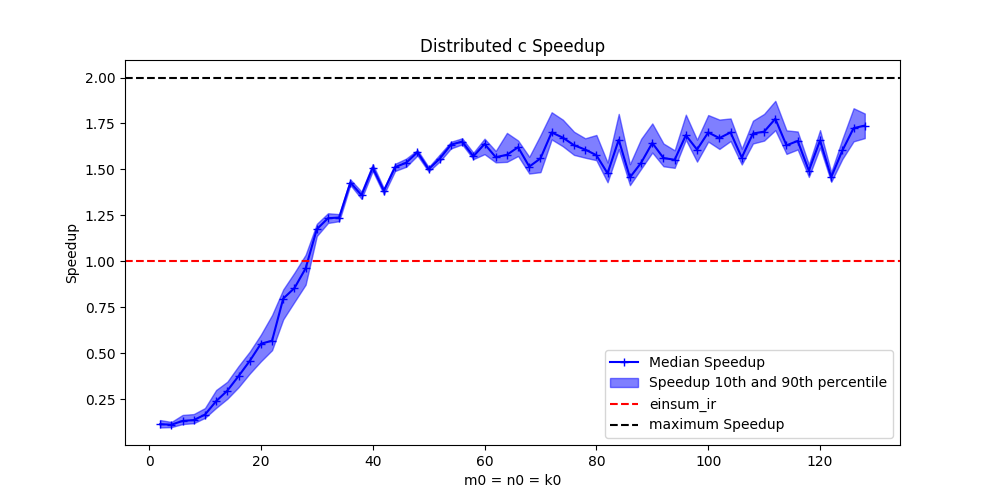
\includegraphics[width=0.95\textwidth]{speedup_c.png}
  }
  \caption{
    Performance and Speedup of the distributed c dimension algorithm compared to \texttt{einsum\_ir} on a 2 socket Nvidia Grace CPU Superchip.
    The contraction is $m_0c_0k_0k_1m_1, n_0c_0k_0n_0n_1 \rightarrow m_0n_0c_0n_1m_1$ with $|c_0|=2$, $|m_0|=|n_0|=|k_0|$ and $|m_1|=|n_1|=|k_1|=70=\texttt{\#compute threads}$.
    $c_0$ got distributed over both cpu chips.
    }
  \label{c_perf}
\end{figure}

\begin{figure}
  \centering{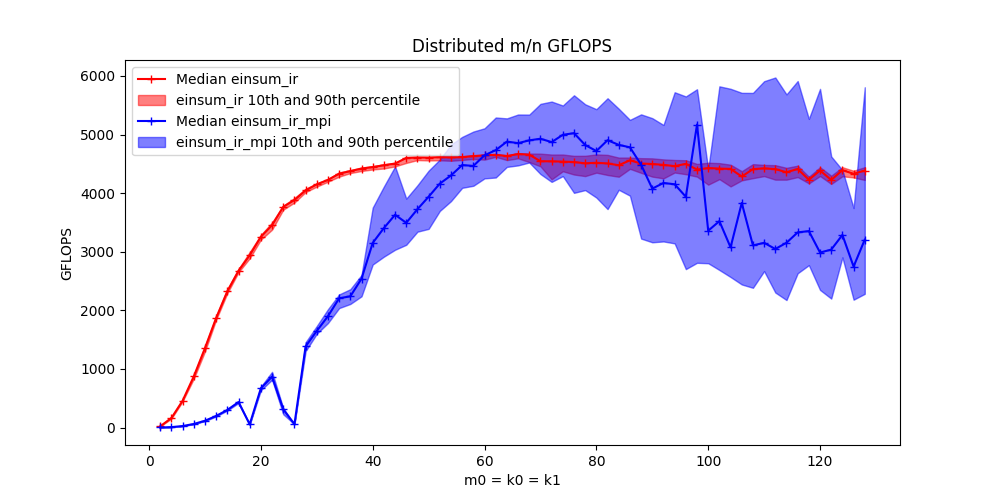
\includegraphics[width=0.95\textwidth]{gflops_m_n.png}
  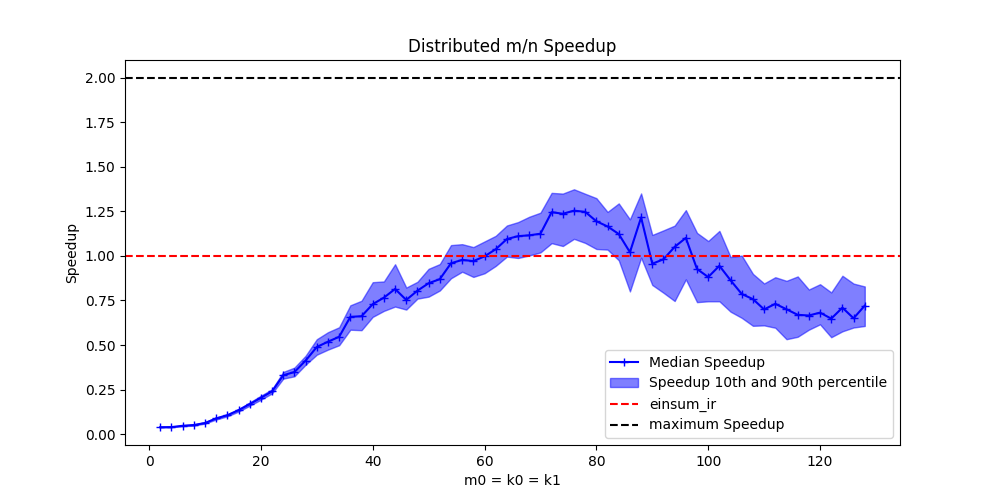
\includegraphics[width=0.95\textwidth]{speedup_m_n.png}
  }
  \caption{
    Performance and Speedup of the distributed m/n dimension algorithm compared to \texttt{einsum\_ir} on a 2 socket Nvidia Grace CPU Superchip.
    The contraction is $m_0c_0k_0k_1m_1, n_0c_0k_0n_0n_1 \rightarrow m_0n_0c_0n_1m_1$ with $|c_0|=2$, $|m_0|=|n_0|=|k_0|$ and $|m_1|=|n_1|=|k_1|=70=\texttt{\#compute threads}$.
    $m_0$ and $n_0$ got distributed over both cpu chips.
    }
  \label{m_n_perf}
\end{figure}

\begin{figure}
  \centering{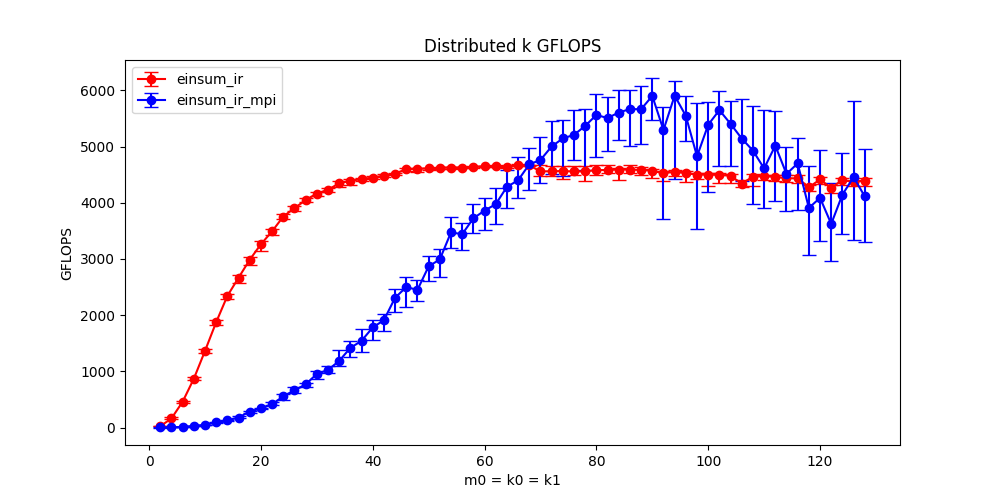
\includegraphics[width=0.95\textwidth]{gflops_k.png}
  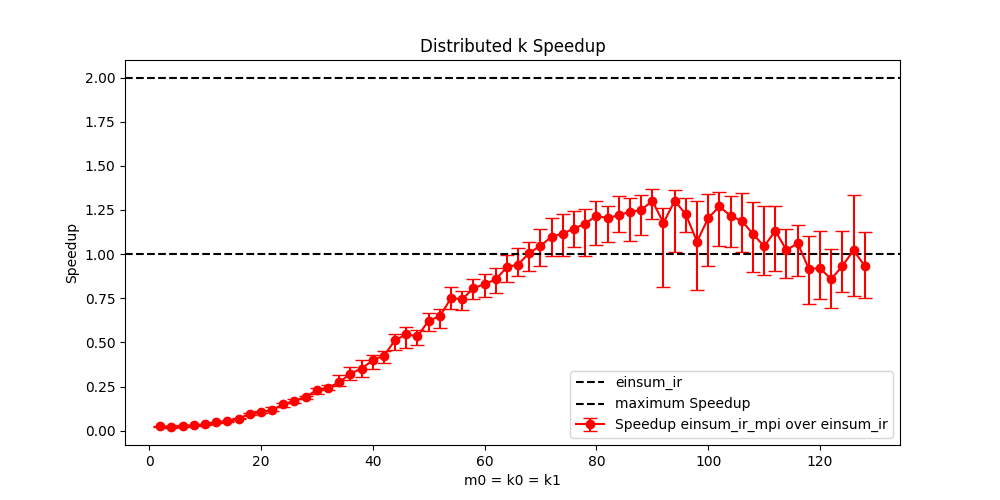
\includegraphics[width=0.95\textwidth]{speedup_k.png}
  }
  \caption{
    Performance and Speedup of the distributed k dimension algorithm compared to \texttt{einsum\_ir} on a 2 socket Nvidia Grace CPU Superchip.
    The contraction is $m_0c_0k_0k_1m_1, n_0c_0k_0n_0n_1 \rightarrow m_0n_0c_0n_1m_1$ with $|c_0|=2$, $|m_0|=|n_0|=|k_0|$ and $|m_1|=|n_1|=|k_1|=70=\texttt{\#compute threads}$.
    $k_0$ got distributed over both cpu chips.
    }
  \label{k_perf}
\end{figure}